\section{Results}
\label{sec:results}

\subsection{Infection estimates and cases-to-infections ratios across the \US states}
\label{sec:omitted-waves}

Prior to Omicron, the largest infection outbreaks were
observed in the late summer and early fall of 2021 in Louisiana, Georgia, Idaho,
and Montana (\Crefrange{fig:state_infect_est}{fig:six-states}). During this time, 
the state with the highest rate of infections on a single day is Louisiana, 
with 476 infections per 100K on July 20, 2021. For comparison, 
the state's 7-day average case rate peaks at 126 cases per 100K on August 13, 2021. 
Idaho follows with an infections peak of 457 per 100K on September 7, 2021, 
and a case peak of 76 per 100K occurring shortly thereafter on September 13, 2021. 
The period of lowest viral transmission is observed in the summer of 2020, when 
Vermont has fewer than 10 infections per 100K per week from June to August, the
 longest such lull observed for any state. %\attn{Can you put one sentence that compares these to the case
%peaks around the same time, just for context?}

\begin{figure}[!tb]
\centering
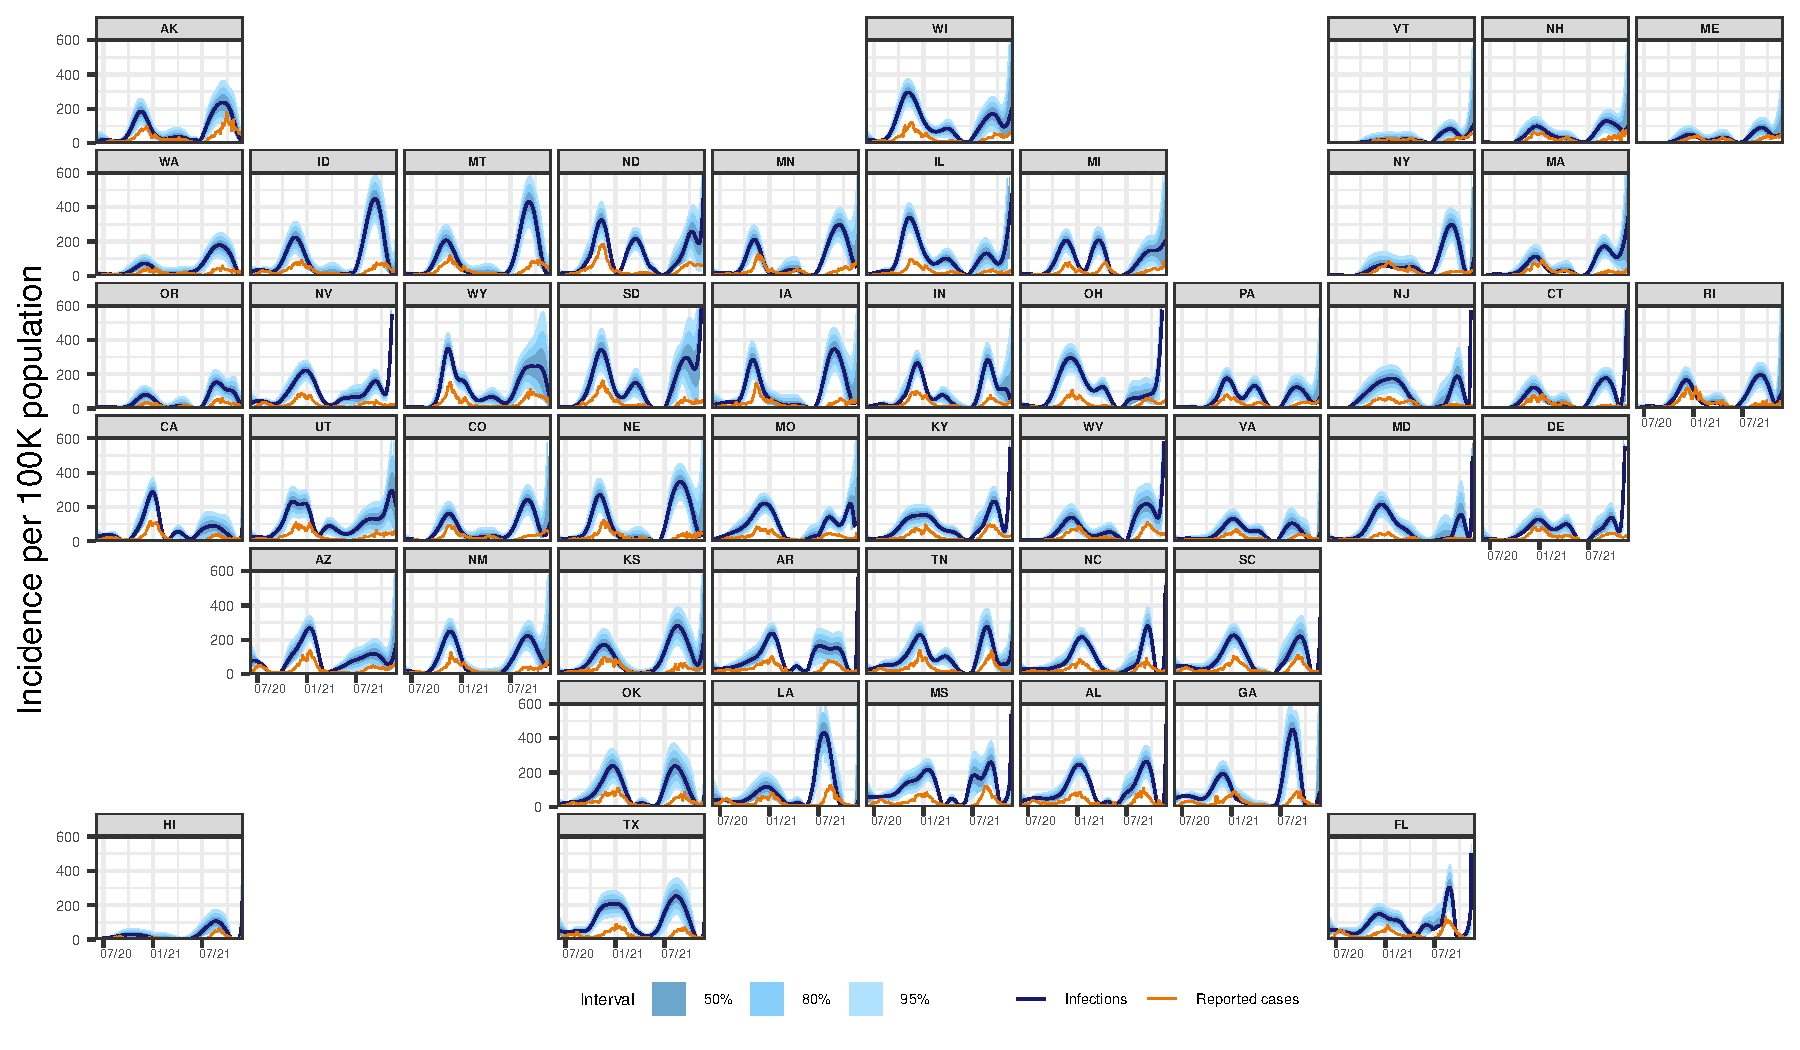
\includegraphics[width=.99\linewidth]{adj-unadj-cases-plot-1.pdf} 
\caption{Estimates of the daily new infections per 100,000 population
for each \US state from June 1, 2020 to November 29, 2021 (dark blue line). The
blue shaded regions depict the 50, 80, and 95\% intervals for the estimates,
while the orange line represents the trailing 7-day average of reported cases
per 100,000.}
\label{fig:state_infect_est}
\end{figure}    

\begin{figure}[!tb]
\centering
    \includegraphics*[width=\linewidth]{six-decon-var-1.pdf}
    \caption{Panel A: Reported cases (orange) and estimates of daily new
    infections (dark blue) per 100K inhabitants. The blue shaded regions
    indicate 50, 80, and 95\% confidence bands.  
    Panel B: Deconvolved cases colored by variant per 100K inhabitants.}
    \label{fig:six-states}
\end{figure}

Nearly all states exhibit two major waves in infections---the Ancestral wave
began in the fall of 2020 and extended into the winter season, while the Delta
wave started in the late summer of 2021 and continued into mid-fall. In general,
greater similarities in the strength and magnitude of outbreaks emerge in small
clusters of states that border each other (Idaho and Montana; North and South
Carolina) present waves of infections that mirror each other in amplitude and
timing.

While the Ancestral, Alpha, and Delta waves are visible for most states, there
are clear outbreaks in unreported infections that are not easily detectable from
cases alone. For example, a wave of infections is evident in North and South
Dakota over the spring of 2021 that is virtually undetectable from reported
cases. Similarly, in late-summer 2021, the Delta wave is only faintly
detectable from cases in a number of Northeastern states, while infections
suggest that it has already begun in earnest.  

Moreover, cases tend to severely underestimate infections during Delta for many
states, more so than in earlier waves (\Cref{fig:state_infect_est}). The most
extreme was New Jersey, where about 6.3\% of estimated infections were
eventually reported as cases. Similarly low are Maryland (7.3\%), Nevada
(8.4\%), and South Dakota (10.0\%). In 44 states, fewer than 1/3 of infections
eventually appear in case reports. The cases-to-infections ratio was larger in
earlier waves, and its effects were most apparent in different regions. During
Alpha, Louisiana had the lowest ratio of infections to cases (11.9\%) followed
by California (13.6\%). Such patterns are less apparent during the Ancestral
wave, where Ohio and Maryland had the lowest ratio of reported cases to
infections at 21.4\% and 21.7\%, respectively. 

\Cref{fig:choro_inf_case_rates} shows that using cases as a proxy for infections
can lead to misunderstandings in the locations that are affected and the extent
to which they are affected. For example, on October 20, 2020, while case rates
are elevated in a handful of upper-Midwestern states (namely, North and South
Dakota), infection rates are elevated to a similar extent in the surrounding
states as well, indicating a wider impact than suggested by cases alone. On July
20, 2021, while the map of case rates shows low and geographically consistent
impact, infection rates reveal that Texas, Louisiana, Georgia, and their
neighbors are hotspots. 
 
By focusing on states with elevated cases, infection outbreaks may be
overlooked. For instance, on August 27, 2021, Montana and Idaho have some of the
highest infection rates (\Cref{fig:choro_inf_case_rates}). In contrast, their
case rates are unremarkable (the highest case rates tend to be in the
Southeast). Infection outbreaks tend to precede case outbreaks, though the lead
time can vary widely. During the Delta wave, infections in Montana 
peaked about 41 days before cases, while in Idaho, they peaked about 6 days before cases
(\Cref{fig:state_infect_est}). During the Ancestral wave, 
infections peaking about 12 days earlier than cases in Montana and 24 days earlier in Idaho,
demonstrating a notable shift in lead times.
%Such
%trends are also observed during the Ancestral wave, where infections peak about
%12 and 24 days earlier than cases for these same states. \attn{These last two
%sentences read strangely: ``41 and 6 days''? what does that mean?} These temporal
%discrepancies underscore the importance of clearly distinguishing between
%infections and cases when assessing the disease burden and spread of COVID-19.

\begin{figure}[H]
\centering
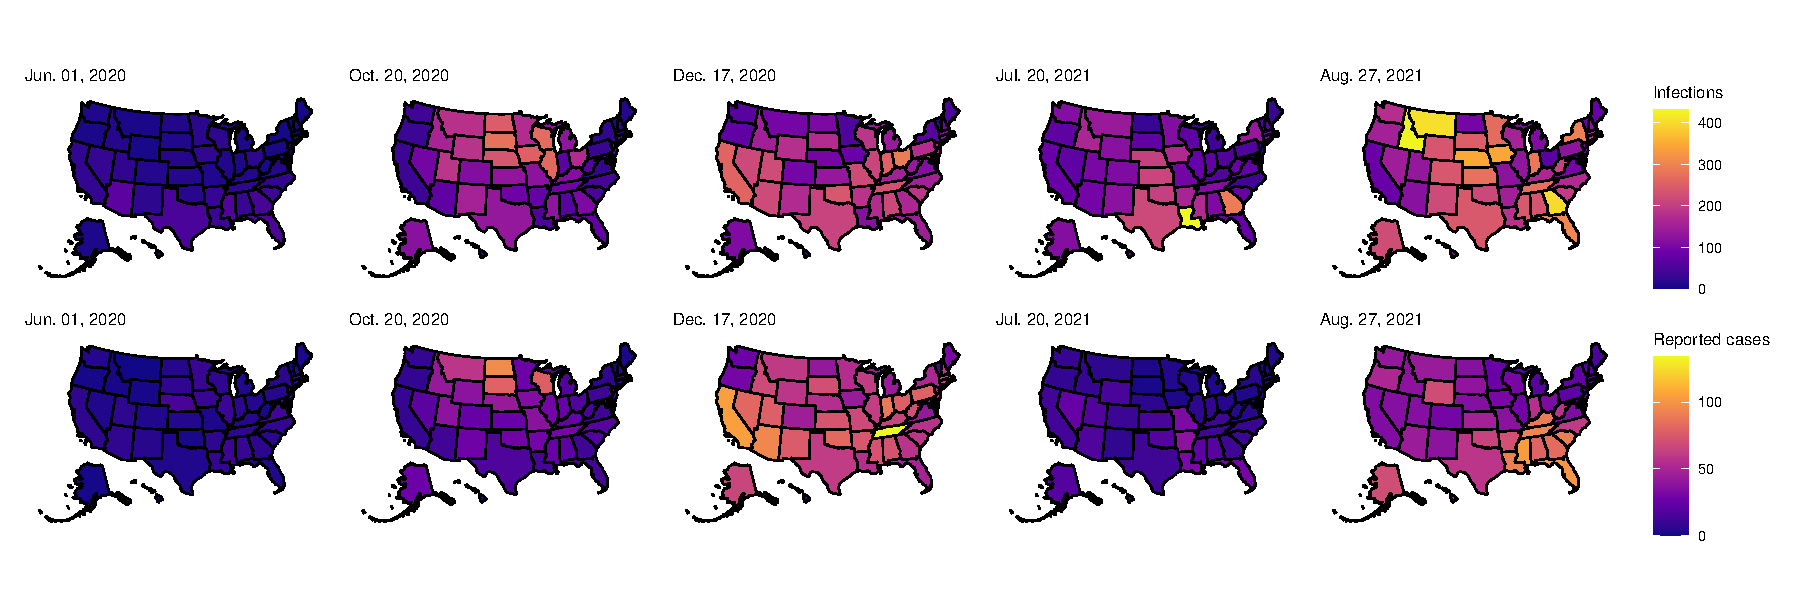
\includegraphics[width=.99\textwidth]{choro-maps-1.pdf}
\caption{Choropleth maps of the state-level estimates of the daily new
infections per 100K (top row) and the daily new cases per 100K (bottom row) for
five select dates between June 1, 2020 and November 29, 2021. Note that the
first date was chosen as a baseline, while the other dates were chosen because
they present large counts of infections across all states. In particular, the
third and fifth dates present the largest number of total infections across the
50 states within those calendar years.} %Note that
%the colors are scaled differently for infections and cases to enable relative comparisons.} 
\label{fig:choro_inf_case_rates}
\end{figure}    

\begin{figure}[H]
\centering
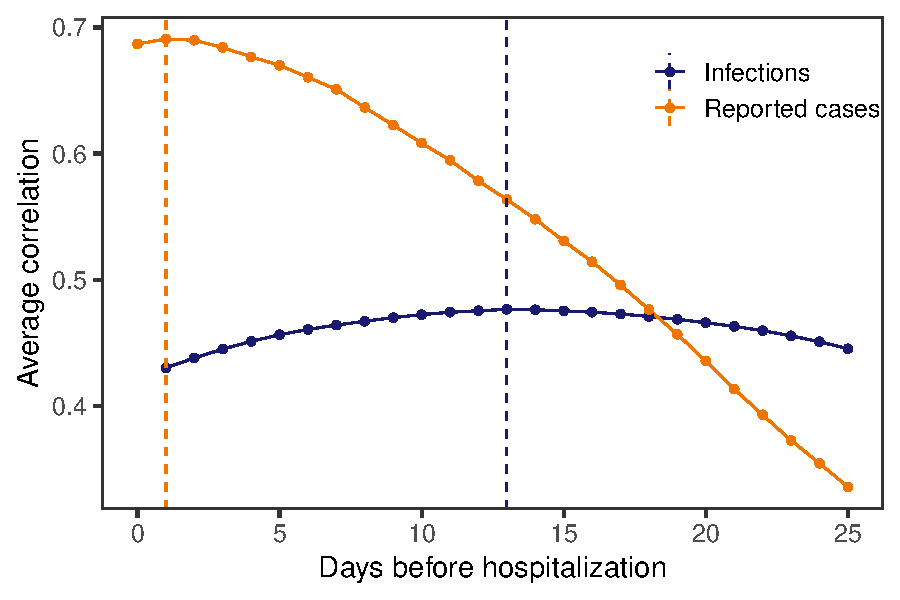
\includegraphics[width=.72\linewidth]{corr-plot-1.pdf} 
\caption{Spearman's rank correlation between each of 
infections and cases with hospitalizations per 100,000. A rolling window of 61 days
 is applied before averaging across all states and times for each lag.
The vertical dashed lines
indicate the lags for which the highest average correlation is attained.}
\label{fig:correlations}
\end{figure}

\begin{figure}[H]
\centering
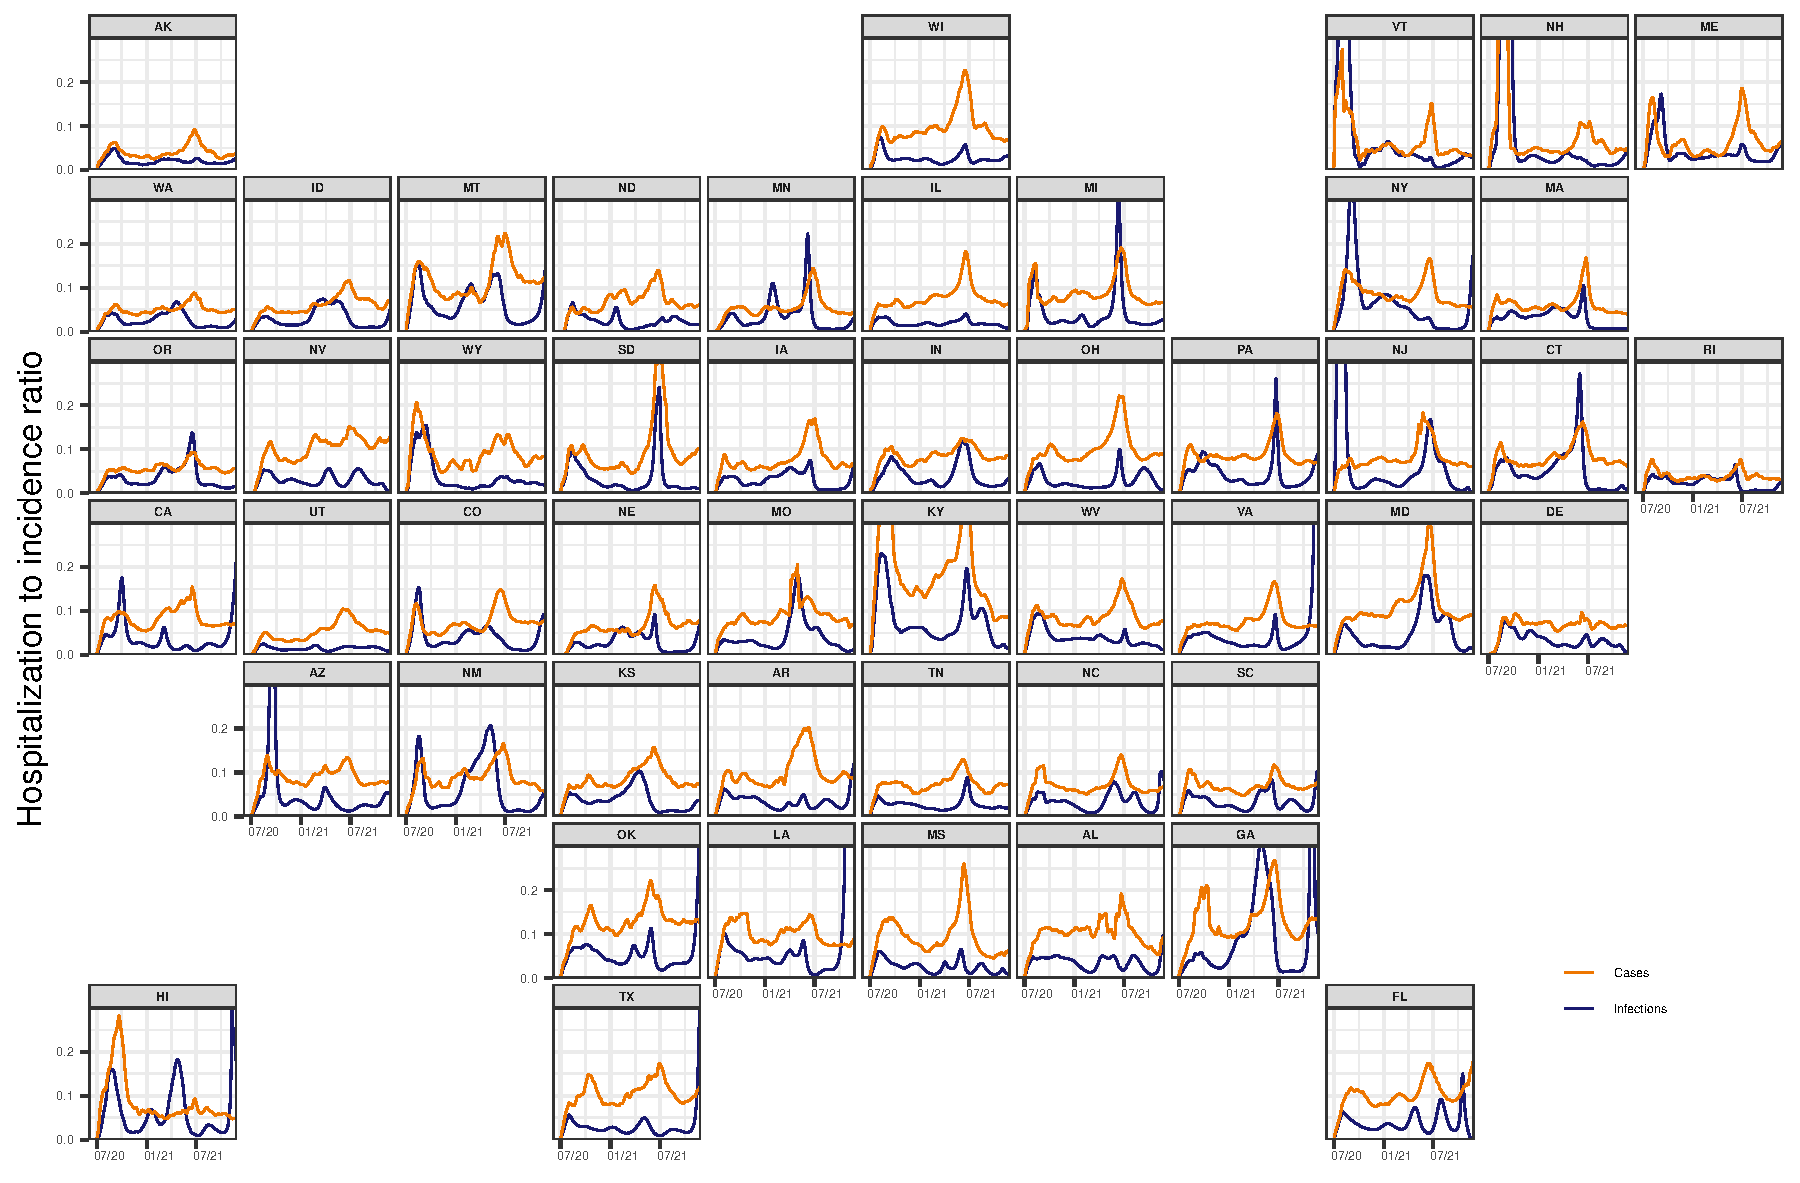
\includegraphics[width=\linewidth]{ihrs-1.pdf}
\caption{Time-varying IHR and CHR estimates for each state from June 1, 2020 to
November 29, 2021, obtained using the respective correlation maximizing lag from
\Cref{sec:lagged-correlations}. Note that the infection, case, and
hospitalization counts are subject to a center-aligned 7-day average to remove
spurious day of the week effects. Also note that the different starting points
across states are due to the availability of the hospitalization data.}
\label{fig:IHR_7dav}
\end{figure} 

\subsection{Insights from cross-correlations, IHRs and CHRs}
\label{sec:lagged-correlations}

%\attn{Need a connecting sentence here. Is this next sentence about infections?}
The maximum Spearman's correlation between infections and hospitalizations
is 0.48 and occurs at a lag of 13 days (\Cref{fig:correlations}). 
In contrast, we find that the
largest average Spearman correlation for cases is 0.69 and occurs at a lag of 1
day. That is, case reports are nearly contemporaneous to hospitalizations, while
infection estimates clearly precede them. 

We compute the time-varying infection-hospitalization ratios (IHRs) for each
state using a 13-day lag and case-hospitalization ratios (CHRs) with a 1-day lag
for comparison \Cref{fig:IHR_7dav}). Overall, the relationship between
infections and hospitalizations is complex. It is characterized by intermittent
spikes that punctuate longer periods where the IHRs are relatively stable,
remaining below 0.1 hospitalizations per infection. 

Both IHRs and CHRs exhibit similar spatiotemporal trends as those noted
for infections. Namely, states that are proximate (for example, North and South
Carolina) show similar temporal patterns in IHRs and CHRs. In addition, similar
spikes are evident across many states during waves of infections that are driven
by variants of concern. For example, many states exhibit a striking increase in
hospitalizations in mid-2021, which coincides with the rapid takeover of the
Delta variant \citep{hodcroft2021covariants}.





